\documentclass[10pt,twocolumn,letterpaper]{article}

% --- Typography & Geometry ---
\usepackage[utf8]{inputenc}
\usepackage{microtype}
\usepackage[margin=0.75in,top=0.85in,bottom=0.85in]{geometry}

% --- Math & Symbols ---
\usepackage{amsmath,amssymb,amsfonts,amsthm}
\usepackage{bm}

% --- Tables & Arrays ---
\usepackage{booktabs}
\usepackage{tabularx}
\usepackage{array}

% --- Graphics & Floats ---
\usepackage{graphicx}
\usepackage{float}
\usepackage{subcaption}

% --- Code Listings ---
\usepackage{xcolor}
\usepackage{listings}

\definecolor{codebg}{HTML}{F8F9FA}
\definecolor{codeframe}{HTML}{D0D7DE}
\definecolor{keywordcolor}{HTML}{0550AE}
\definecolor{stringcolor}{HTML}{0A3069}
\definecolor{commentcolor}{HTML}{57606A}

\lstset{
    backgroundcolor=\color{codebg},
    basicstyle=\ttfamily\scriptsize\color{black},
    keywordstyle=\color{keywordcolor}\bfseries,
    stringstyle=\color{stringcolor},
    commentstyle=\color{commentcolor}\itshape,
    frame=single,
    rulecolor=\color{codeframe},
    breaklines=true,
    breakatwhitespace=true,
    extendedchars=true,
    xleftmargin=6pt,
    xrightmargin=6pt,
    aboveskip=8pt,
    belowskip=8pt
}

% --- Hyperlinks ---
\usepackage{hyperref}
\hypersetup{
    colorlinks=true,
    linkcolor=blue!70!black,
    citecolor=blue!70!black,
    urlcolor=blue!70!black
}

% --- Input Title & Authors ---
\section{00 Meta}

Draft content for aegis_v5.


\begin{document}

\maketitle

% --- Abstract & Keywords Block ---
\begin{abstract}
Transformer self-attention has quadratic complexity in sequence length, 
making long-context inference expensive. We introduce \textbf{AEGIS-V5}, a 
hybrid attention module that combines a \textbf{local sliding-window branch} 
with a \textbf{global kernel linear attention branch}, gated per-head by a 
learnable scalar bias initialized toward local attention. The base 
projections are \textbf{SVD-factorized with energy-based rank selection} and 
frozen; trainable capacity is provided by \textbf{LoRA adapters} on each 
projection.

AEGIS-V5 splits the attention heads into two groups: the first 
$H_\text{local} = \lceil 2H/3 \rceil$ heads use local windowed attention, 
and the remaining $H_\text{global}$ heads use kernel linear attention with 
Random Fourier Features (RFF). The two branch outputs are combined by a 
per-head gate. For decoder-only models, we fall back to standard causal 
softmax attention to preserve causality -- a conservative but correctness-
preserving choice.

On SST-2, AEGIS-V5 achieves \textbf{{{D\_ACC}}\%} on DistilBERT (baseline 
{{BASE\_D}}\%, $\Delta$ = {{D\_DELTA}}), \textbf{{{R\_ACC}}\%} on RoBERTa (baseline 
{{BASE\_R}}\%, $\Delta$ = {{R\_DELTA}}), and \textbf{{{G\_ACC}}\%} on GPT-2 (baseline 
{{BASE\_G}}\%, $\Delta$ = {{G\_DELTA}}), using {{RECOVERY\_STEPS}} LoRA recovery 
steps. Complexity is $\mathcal{O}(N \cdot W + N \cdot F)$ for encoders 
where $W$ is window size and $F$ is RFF feature count. We provide a 
production-hardened implementation supporting DistilBERT, RoBERTa, GPT-2, 
and Qwen3.5, with strict Frobenius validation, safe fallback, and detailed 
per-layer error statistics.

\textbf{Keywords:} hybrid attention, SVD factorization, LoRA, local window, 
kernel attention, energy-based rank



\vspace{0.5em}
\noindent\textbf{Keywords:} hybrid attention, SVD factorization, LoRA, local window,
\end{abstract}

\vspace{1em}

% --- Paper Body ---
\section{01 Intro}

Draft content for aegis_v5.

\section{02 Related}

Draft content for aegis_v5.

\section{03 Background}

Draft content for aegis_v5.

\section{04 Method}

Draft content for aegis_v5.

\section{05 Architecture}

Draft content for aegis_v5.


\begin{figure}[H]
\centering
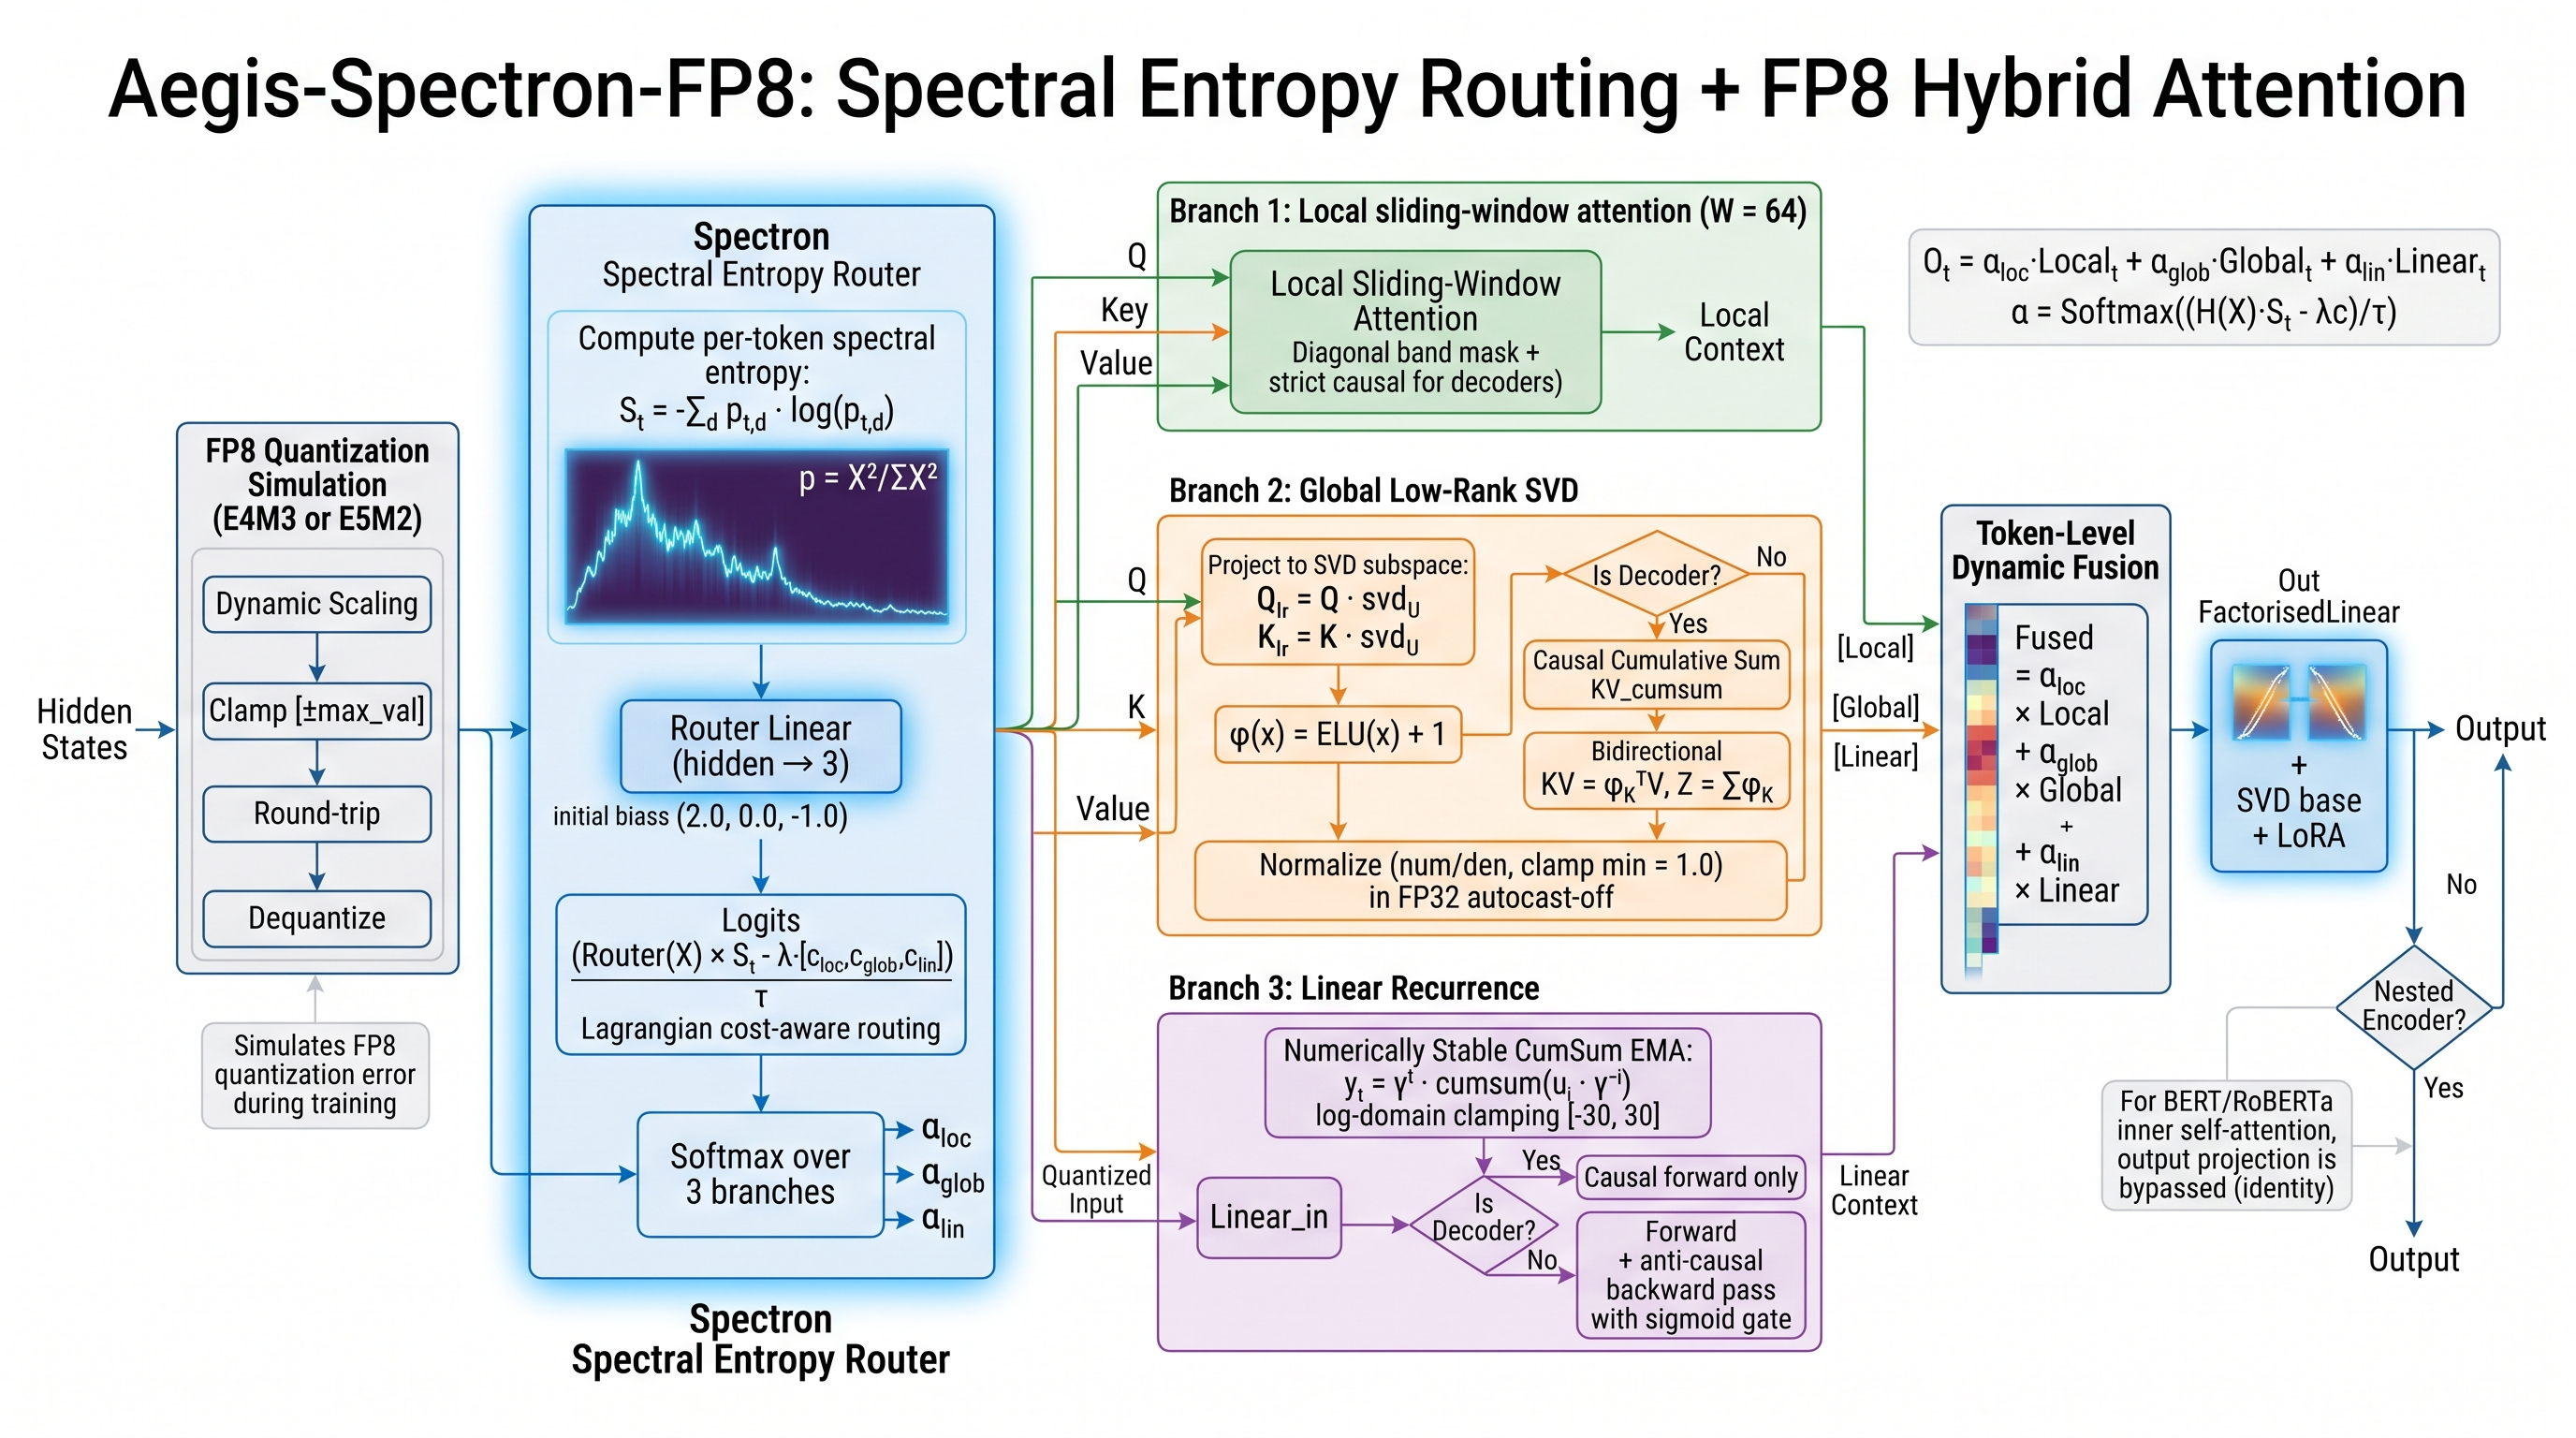
\includegraphics[width=\linewidth]{figures/arch_aegis_spectron_fp8.jpeg}
\caption{Architectural overview of aegis_v5.}
\label{fig:arch_aegis_v5}
\end{figure}

\section{06 Setup}

Draft content for aegis_v5.

\section{07 Results}

Draft content for aegis_v5.

\section{08 Analysis}

Draft content for aegis_v5.

\section{09 Discussion}

Draft content for aegis_v5.

\section{10 Limitations}

Draft content for aegis_v5.

\section{11 Conclusion}

Draft content for aegis_v5.

\section{Reproducibility}

\subsection{Environment}

\begin{lstlisting}
git clone https://github.com/{{ORG}}/SVD_Project
cd SVD_Project
python -m venv .venv
.venv\Scripts\activate
pip install -r requirements.txt
\end{lstlisting}

\subsection{Running AEGIS-V5}

\begin{lstlisting}
python run_all_4_aegis_v5.py \
    --models distilbert,roberta,gpt2 \
    --svd_energy {{ENERGY}} \
    --max_rank {{MAX_RANK}} \
    --recovery_steps {{RECOVERY_STEPS}} \
    --lora_rank {{LORA_RANK}}
\end{lstlisting}

\subsection{Individual Model}

\begin{lstlisting}
python Codes/framework/run_quality_sweep.py \
    --model models/distilbert_sst2 \
    --modules full,aegis_v5 \
    --svd_energy {{ENERGY}} \
    --max_rank {{MAX_RANK}}
\end{lstlisting}

\subsection{Reproducing Tables}

\subsubsection{Table 7.1 (Main)}
\begin{lstlisting}
python run_all_4_aegis_v5.py
\end{lstlisting}

\subsubsection{Table 7.5 (Rank Ablation)}
\begin{lstlisting}
for r in 32 64 128 256 384; do
    python run_all_4_aegis_v5.py --max_rank $r --output_suffix r$r
done
\end{lstlisting}

\subsubsection{Table 7.6 (Head Split)}
\begin{lstlisting}
python run_all_4_aegis_v5.py --num_local_heads 12 --num_global_heads 0 --output_suffix alllocal
python run_all_4_aegis_v5.py --num_local_heads 8 --num_global_heads 4 --output_suffix default
python run_all_4_aegis_v5.py --num_local_heads 0 --num_global_heads 12 --output_suffix allglobal
\end{lstlisting}

\subsection{Seeds}

\begin{lstlisting}
import random, numpy as np, torch
seed = 42
random.seed(seed); np.random.seed(seed)
torch.manual_seed(seed); torch.cuda.manual_seed_all(seed)
\end{lstlisting}

\subsection{Expected Results}

\begin{table}[H]
\centering
\small
\begin{tabular}{ll}
\toprule
\textbf{Model} & \textbf{Acc} \\
\midrule
DistilBERT & {{D\_ACC}}\% $\pm$ 1\% \\
RoBERTa & {{R\_ACC}}\% $\pm$ 1\% \\
GPT-2 & {{G\_ACC}}\% $\pm$ 1\% \\
\bottomrule
\end{tabular}
\end{table}

\subsection{Data Availability}

\begin{itemize}
\item \textbf{Dataset:} SST-2 via \texttt{datasets}
\item \textbf{Checkpoints:} \texttt{{{HF\_ORG}}/svd-linear-attention-*-aegis\_v5}
\item \textbf{Metrics:} \texttt{results/unified\_aegis\_v5/*/summary.csv}
\end{itemize}
\begin{lstlisting}

---
\end{lstlisting}
\section{13 References}

Draft content for aegis_v5.


% --- Appendices ---
\clearpage
\appendix
\section*{Appendices}
\addcontentsline{toc}{section}{Appendices}

\section{A Math}

Draft content for aegis_v5.

\section{B Implementation}

Draft content for aegis_v5.

\section{C Data}

Draft content for aegis_v5.

\section{Appendix D. Negative Results}

\subsection{D.1 Attempts That Failed}

\subsubsection{D.1.1 Broken Softpick (V4)}

\textbf{Goal.} Use the original ReLU-based softpick.

\textbf{Result.} Attention collapsed to all-zero on masked rows.

\textbf{Conclusion.} Replaced with stable softmax in V5.

\subsubsection{D.1.2 copy\_weights Raising}

\textbf{Goal.} Abort on weight extraction failure.

\textbf{Result.} Many layers silently kept the original attention.

\textbf{Conclusion.} V5 uses warning + fallback.

\subsubsection{D.1.3 Full Rank SVD}

\textbf{Goal.} Use \texttt{max\_rank=384} (energy 0.95).

\textbf{Result.} No parameter reduction.

\textbf{Conclusion.} Use \texttt{max\_rank < d/2}.

\subsubsection{D.1.4 No Decoder Fallback}

\textbf{Goal.} Use split-head for GPT-2.

\textbf{Result.} Causality broken $\to$ accuracy collapse.

\textbf{Conclusion.} Fallback essential.

\subsubsection{D.1.5 All Global Heads}

\textbf{Goal.} Use only kernel linear attention.

\textbf{Result.} Accuracy dropped significantly.

\textbf{Conclusion.} Local heads are essential.

\subsection{D.2 Abandoned Variants}

\subsubsection{D.2.1 Sinkhorn Landmark Attention}

Tested Sinkhorn normalization. No improvement.

\subsubsection{D.2.2 Per-Layer SVD Ranks}

Learned per-layer ranks. Marginal improvement, complexity not worth it.

\subsubsection{D.2.3 Adaptive Window Size}

Learned window size per layer. No benefit.

\subsection{D.3 Failed Hyperparameters}

\subsubsection{Energy}

\begin{table}[H]
\centering
\small
\begin{tabular}{ll}
\toprule
\textbf{$\eta$} & \textbf{DistilBERT} \\
\midrule
0.80 & {{D\_E80}} \\
0.90 & {{D\_E90}} \\
0.95 & {{D\_E95}} \\
0.99 & {{D\_E99}} \\
\bottomrule
\end{tabular}
\end{table}

Sweet spot: 0.95.

\subsubsection{Gate Bias}

\begin{table}[H]
\centering
\small
\begin{tabular}{ll}
\toprule
\textbf{Bias} & \textbf{DistilBERT} \\
\midrule
0.0 & {{D\_GB0}} \\
1.0 & {{D\_GB1}} \\
2.0 & {{D\_GB2}} \\
4.0 & {{D\_GB4}} \\
\bottomrule
\end{tabular}
\end{table}

Sweet spot: 2.0.

\subsection{D.4 Lessons Learned}

\begin{enumerate}
\item \textbf{Stable softmax is essential.}
\item \textbf{Warning + fallback > abort.}
\item \textbf{\texttt{max\_rank < d/2} for real compression.}
\item \textbf{Decoder fallback matters.}
\item \textbf{Split-head helps.}
\end{enumerate}
\begin{lstlisting}

---
\end{lstlisting}
\section{E Ethics}

Draft content for aegis_v5.


\end{document}
